\chapter {Introduzione}

Nella parte che segue sarà studiata l’aerodinamica del profilo laminare $66_4-221$ appartenente alla sesta serie NACA.\\
La sigla caratterizzante il profilo contiene le caratteristiche principali dello stesso, riassunte nel seguente schema \\

\begin{figure} [h!]
\centering
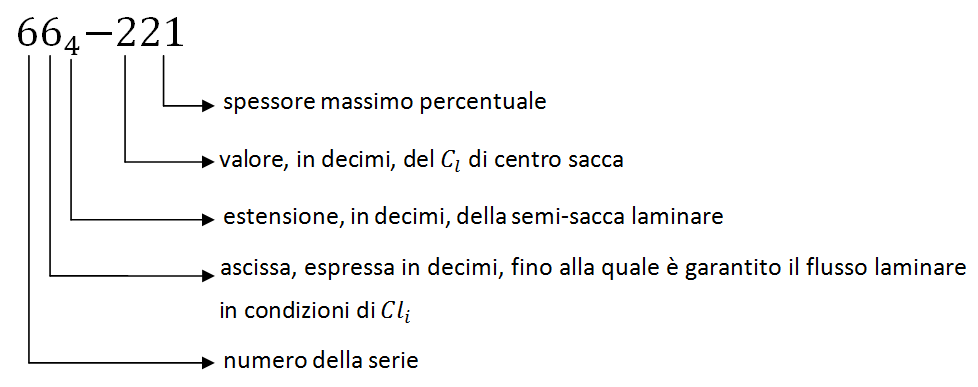
\includegraphics  [ height=6cm] {immagini/laminare.png}
\caption{\footnotesize Significato cifre profilo laminare NACA $66_4-221$ }
\label{fig:lamin}
\end{figure}

\noindent \\

Di seguito saranno svolti sul detto profilo i medesimi studi effettuati nella {\itshape Parte I} relativamente al profilo {\bfseries SELIG 4110}, pertanto, in questa sede, saranno limitate al massimo eventuali spiegazioni non strettamente necessarie.\\
In primo luogo verrà trattata la geometria del profilo, e la relativa costruzione. In seguito verranno ricavate le caratteristiche geometriche dello stesso e i risultati del profilo sottile. Sará poi studiata la soluzione in campo Euleriano incomprimibile a vari $C_l$ significativi, graficandone il coefficiente di pressione e la soluzione in campo viscoso introducendo,quindi, gli effetti del numero di Reynolds.
